\begin{figure*}
% [htp]
  \centering
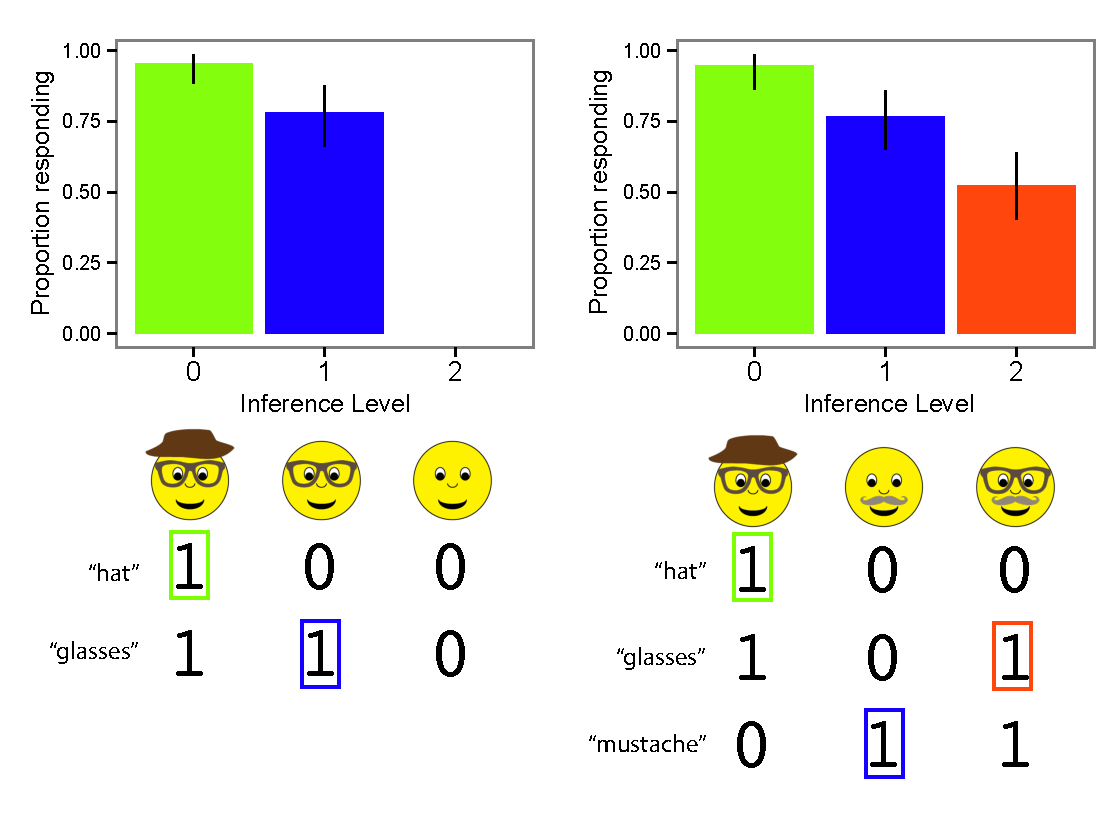
\includegraphics[width=4.75in]{fig/ann-ibr-bargraph.pdf}
\caption{\label{fig:humans} Human data and experimental matrices from Experiments 1 and 2.}
\end{figure*}

\begin{figure*}[t]
  \centering
  \subfigure[ANN Simple]{
    \centering
    \includegraphics[width=0.8\columnwidth]{fig/scales.pdf}
    \label{fig:scales}
  } 
  \hspace{40pt}
  \subfigure[ANN Complex]{
    \centering
    \includegraphics[width=0.8\columnwidth]{fig/scalesPlus.pdf}
    \label{fig:scalesPlus}
  }
  \caption{Evaluation of the ANN listener with 50 hidden nodes on the simple (a) and complex (b) settings.}

  \subfigure[IBR Simple]{
    \centering
    \includegraphics[width=0.8\columnwidth]{fig/IBRscales.pdf}
    \label{fig:ibrScales}
  } 
  \hspace{40pt}
  \subfigure[IBR Complex]{
    \centering
    \includegraphics[width=0.8\columnwidth]{fig/IBRscalesPlus.pdf}
    \label{fig:ibrScalesPlus}
  }
  \caption{Evaluation of IBR listeners with different depths of recursion.}
\end{figure*}


%\begin{figure}
%    \includegraphics[width=\columnwidth]{fig/hiddenscales.pdf}
%    \caption{\label{fig:hiddenScales}ANN accuracy with a varying number of hidden nodes on the simple condition.}
%\end{figure}
%\begin{figure}
%    \includegraphics[width=\columnwidth]{fig/hiddenscalesPlus.pdf}
%    \caption{\label{fig:hiddenScalesPlus}ANN accuracy with a varying number of hidden nodes on the complex condition.}
%\end{figure}


\section{Experiment 1: Simple Scalar Implicature}

To quantitatively compare our model with human data, we conducted two
experiments with human participants in which we asked them to play
reference games that varied in their inferential complexity. We then
compare performance of human participants to that of our
discriminative model. Our first experiment used the simple referential
context shown in the left of Figure \ref{fig:humans}, following
\cite{Stiller:Goodman:Frank:2011}.

\subsection{Methods}

\subsubsection{Participants}

We recruited 120 participants on Amazon Mechanical Turk, of whom 65
received the level 0 stimulus, and 55 received the level 1 stimulus.

\subsubsection{Stimuli}

For each participant, we generated a reference game with an underlying
matrix description identical to that shown in the left of
Figure~\ref{fig:humans}. We generated the reference game by choosing a
base item randomly from among six possible options: boat, friend
(shown in Figure~\ref{fig:humans}), pizza, snowman, sundae, and
Christmas tree. Each of the possible items had three features that
were plausible additions to the base item. For example, the friend
item has a hat, glasses, and mustache, while the boat item has a sail,
cabin, and motor. For this experiment, we randomly chose two features,
randomly assigning them to rows in the underlying matrix (ensuring,
e.g., that glasses was not always the target feature), and we randomly
assigned targets to positions in the display (ensuring, e.g., that the
target was not always in the middle).

This reference game supports two possible inference types, which we
refer to as ``level 0'' and ``level 1'', following our usage in the
previous section.  In the case of the display shown in
Figure~\ref{fig:humans}, the message ``hat'' unambiguously refers to
the face with the hat and glasses; since there is no inference
necessary, we call this a ``level 0'' problem. In contrast, the
message ``glasses'' could logically refer to the face with a hat and
glasses, or the face with just a hat. A pragmatic inference is
required to conclude that the message refers to the face
\emph{without} a hat; we refer to this as a ``level 1'' problem.


\subsubsection{Procedure}

Participants saw a webpage that first introduced them to an
interlocutor, ``Bob'', who routinely engaged in some action (e.g.,
visiting his friends for the friend item). They then saw a scene like
that shown in Figure~\ref{fig:humans} and read that ``Bob can only say
one word to communicate with you and he says: [target]'', where
[target] indicates the message relating to the particular condition
they had been randomly assigned to (e.g., ``glasses'' for the level~1
inference in Figure~\ref{fig:humans}).  Participants were instructed
to indicate which item they thought was Bob's target via a
3-alternative forced-choice. Afterwards, they completed a simple check
question (provide the interlocutor's name), which we used to exclude
non-compliant participants.

\subsection{Results}

Human performance is plotted in the bar graph in
Figure~\ref{fig:humans}. The level~0 utterance was trivial, with 95\%
of participants choosing correctly. Participants also made a
substantial portion of implicature-consistent responses (75\%) in the
level~1 condition, replicating \cite{Stiller:Goodman:Frank:2011}.

We next compare human performance to the ANN listener model, which was
trained on $\Gsep$. The accuracy of an ANN listener with 50 hidden
nodes is shown in Figure~\ref{fig:scales}, for a variety of training
iterations. The case of 0 training iterations corresponds to the
literal listener $L_{0}$. We see that the literal listener gets all of
the level~0 (unambiguous) problems correct, and 50\% of the level~1
problems. The ANN slightly outperforms the humans but is well aligned
with them: 91\% accuracy on the level~0 problems, and 86\% accuracy on
the level~1 problems.

%We also explored the effect the size of the hidden layer has on model performance, displayed in Figure \ref{fig:hiddenScales}. Listeners with very limited hidden layers do not learn the task, but do well after using 15 hidden nodes or more.

Lastly, we evaluated the iterated best response (IBR) model on this
condition, shown in Figure~\ref{fig:ibrScales}. The IBR model is
always correct on the level 0 problems, and quickly increases in
accuracy on the level 1 problems as the depth of recursion
increases. This evaluation uses the IBR probabilities to compute
accuracy. If we instead evaluate by predicting the target with highest
probability for each message, it gets all of the level 1 problems
correct after one level of recursion.


\section{Experiment 2: Complex Scalar Implicature}

\subsection{Methods}

\subsubsection{Participants} 

We recruited 180 participants from Mechanical Turk, with 55 receiving
the level 0 stimulus, 60 receiving level 1, and 65 receiving level 2.

\subsubsection{Stimuli}

Stimuli were generated identically to those in Experiment~1, except
that we used the base matrix shown on the right in
Figure~\ref{fig:humans}. With the setting shown there, the message
``hat'' is level~0, ``mustache'' is level~1, and ``glasses'' is
level~2.

\subsubsection{Procedure}

The procedure was identical to Experiment 1. 

\subsection{Results}

Figure~\ref{fig:humans} shows human performance on the more complex
scalar implicature task. Similar to the simple task, 95\% correctly
identified the level~0 referent, and 77\% correctly picked the level~1
referent. However, humans had much more trouble with the level~2
inference, with just 52\% selecting the correct referent given the
utterance.

These results too align with the ANN model
(Figure~\ref{fig:scalesPlus}). We see similar performance on the
level~0 and level~1 problems as in the previous
experiment. Importantly, the model also has much more difficulty with
the level~2 problems (70\% accuracy), which persists across number of training
iterations. Although the model is more accurate than the human
subjects, the results are qualitatively similar. 

This stands in marked contrast to the IBR model's performance, summarized in
Figure~\ref{fig:ibrScalesPlus}. This model always gets the level~0
problems correct. As the depth of recursion increases, the IBR
confidence asymptotes to 1. In the same way as in the simple
condition, if we instead evaluate the IBR model by choosing the
highest probability target for each message, it correctly identifies
the level~1 targets after one step of recursion, and all of the
level~2 problems after two steps of recursion, thereby vastly
outperforming our human subjects.
